\documentclass[10pt,twoside,titlepage]{article}   % Standard LaTeX
\usepackage{amsmath,amssymb}    % For better support of math
\usepackage{url}
\usepackage{graphicx}          % Enable for eps,jpeg figures

\usepackage{afterpage}

\newcommand\blankpage{%
    \null
    \thispagestyle{empty}%
    \addtocounter{page}{-1}%
    \newpage}

\urldef\HHIURL\url{https://en.wikipedia.org/wiki/Herfindahl%E2%80%93Hirschman_index#Effective_assets_in_a_portfolio}

\DeclareMathOperator*{\argmax}{arg\,max}
\DeclareMathOperator*{\argmin}{arg\,min}

%% Controls spacing between lines (\doublespacing, \onehalfspacing, etc.):
\usepackage{setspace}

%% Use the line below for official NYU version, which requires
%% double line spacing. For all other uses, this is unnecessary,
%% so the line can be commented out.
\doublespacing % requires package setspace, invoked above

\usepackage{listings}
\usepackage{color}

\definecolor{dkgreen}{rgb}{0,0.6,0}
\definecolor{gray}{rgb}{0.5,0.5,0.5}
\definecolor{mauve}{rgb}{0.58,0,0.82}

\lstset{frame=tb,
  language=Python,
  aboveskip=3mm,
  belowskip=3mm,
  showstringspaces=false,
  columns=flexible,
  basicstyle={\small\ttfamily},
  numbers=none,
  numberstyle=\tiny\color{gray},
  keywordstyle=\color{blue},
  commentstyle=\color{dkgreen},
  stringstyle=\color{mauve},
  breaklines=true,
  breakatwhitespace=true,
  tabsize=3
}
% See: https://stackoverflow.com/questions/3175105/inserting-code-in-this-latex-document-with-indentation

\begin{document}

\title{Improved Portfolio Diversification Through Unsupervised Learning}
\author{Michael J. Lewis}
%\date{\copyright\today}         % change \today to a particular date
\date{
Original version: August 6, 2019 \\
This version: August 6, 2023 }

\maketitle
%\afterpage{\blankpage}

\begin{abstract}
This paper introduces the Recursive Clustering Risk Parity (RCRP) approach. 
The RCRP method builds on the philosophy first introduced in Hierarchical Risk Parity (HRP) in \cite{HRP}, leveraging unsupervised learning to recursively build an optimal portfolio. 

HRP established the concept of building a diversified portfolio using the inherent structure of the covariance matrix, utilizing graph theory and hierarchical clustering. In doing so, HRP avoided inverting the covariance matrix, a numerically unstable procedure when performed on the notoriously ill-conditioned, if not singular, empirical covariance matrix in financial applications. However, the procedure relies on sorting the underlying instruments and, in doing so, creating a quasi-diagonalization of the matrix,  thereby foregoing the underlying tree structure. RCRP builds on this premise by utilizing this underlying tree structure, leveraging improved clustering techniques and inversion approximations to enhance overall performance.\\
Keywords: Risk parity, tree graph, cluster, recursive, inverse rank-one update, metric space.\\
JEL Classification: G0, G1, G2.\\
AMS Classification: 91G10, 91G60, 91G70, 60E.\\
\end{abstract}

\section{Portfolio Optimization: A Background}\label{sec-intro}
This paper proposes a method to obtain two desirable portfolios: the minimum variance portfolio and the maximum sharpe ratio portfolio. 
We consider both the case where there are limits on shorts, and when there are not; initially, we will focus on the case without limits.

For completeness, a portfolio is a vector of weights $w$ across $N$ market instruments. 
When considering the case of no shorting limits, the weights sum to unity, or $1^Tw=1$, 
while in the case with limits the absolute weights sum to unity, or $\sum_i |w_i|=1$. 
Given the covariance matrix $\Sigma$, expected excess returns vector $\mu$, and portfolio weights $w$,
the variance of the portfolio is $w^T \Sigma w$ and the expected excess return of the portfolio is $w^T \mu$.
With that terminology in place, we will be discussing the minimum variance portfolio without shorting limits, which satisfies
\begin{equation}\label{MinVarEqn}
\begin{aligned}
\argmin_{w} \quad & w^T \Sigma w \\
\textrm{s.t.} \quad & 1^T w = 1\\
\end{aligned}
\end{equation} 
and the maximum sharpe ratio portfolio without shorting limits, which satisfies
\begin{equation}\label{MaxSharpeEqn}
\begin{aligned}
\argmax_{w} \quad & \frac{w^T \mu}{ \sqrt{ w^T \Sigma w } } \\
\textrm{s.t.} \quad & 1^T w = 1\\
\end{aligned}
\end{equation}

The known optimal solution to equation (\ref{MinVarEqn}) is setting $w=\frac{\Sigma^{-1} 1}{1^T\Sigma^{-1} 1}$, or equivalently $w\propto \Sigma^{-1} 1$, 
whereas the known optimal solution to equation (\ref{MaxSharpeEqn}) is setting $w\propto \Sigma^{-1} \mu$.\footnote{See Appendix \ref{sec-Appendix1} for details} 
Put more concisely, the solutions set $w\propto \Sigma^{-1} b$, where $b=1$ for the minimum variance portfolio, and $b=\mu$ for the max sharpe ratio. 
Unfortunately, both solutions require inverting the covariance matrix, a numerically unstable task when it is possible, 
and impossible when the covariance matrix is singular, as is often the case in practice when involving thousands of stocks. 
Aside from this inherent numerical instability, empirical covariance matrices can themselves be noisy 
when evaluated on a finite number of financial returns, further complicating matters. 
A method that is robust to noise and does not require ill-conditioned matrix inversion is desirable.
 
One notable option for the minimum variance portfolio is the inverse variance portfolio (IVP). 
In this case, the weight $w_i$ given to instrument $i$ is set to be inversely proportional to its variance $\sigma_i^2$, or $w_i \propto \frac{1}{\sigma_i^2}$. 
Observe that this is the optimal solution in the special case where the instruments are independent, 
or equivalently $\Sigma = \Sigma_{diag}$ is a diagonal matrix with $\sigma_{ij} = \Sigma_{ij} = 0$ for $i \neq j$. 
HRP notably uses this result when recursively evaluating the portfolio weights subsequent to quasi-diagonalizing the covariance matrix. 
However, in finance it is often the case that instruments are not independent, and for this reason the inverse variance portfolio is suboptimal.

\section{Improved Inverse Approximation}\label{sec-approx}
A notable improvement to the inverse variance portfolio can be found in \cite{LopezAndLewis}. 
We assume a constant correlation $\rho$ between each instrument $i, j$ with $i \neq j$, then $\sigma_{ij}=\rho \sigma_i \sigma_j$, and thus
\begin{equation*}
\Sigma = (1 - \rho) \Sigma_{diag} + \rho \sigma \sigma^T
\end{equation*}
where $I$ is the identity matrix, and $\sigma$ is the column vector of standard deviations. 
Given this is a rank-one update to the matrix $(1 - \rho) \Sigma_{diag}$, we can use the Sherman-Morrison Identity to evaluate its analytic inverse.
\begin{equation*}
\Sigma^{-1} = \frac{1}{1 - \rho} \Sigma_{diag}^{-1} - \frac{ \rho }{ (1-\rho) (1 + \rho (N-1) ) } \left( \frac{1}{\sigma} \right) \left( \frac{1}{\sigma} \right)^T
\end{equation*}
In this equation $\left( \frac{1}{\sigma} \right)$ is, with slight abuse of notation, 
the vector with component $i$ set to $\frac{1}{\sigma_i}$. 
For a covariance matrix with this form, the optimal minimum variance portfolio takes the form
\begin{equation*}
w_i \propto \frac{1}{\sigma_i^2} - \frac{ \rho \sum_j \frac{1}{\sigma_j} }{ ( 1 + \rho (N-1) )\sigma_i  }
\end{equation*}
while the optimal maximum sharpe ratio portfolio has
\begin{equation*}
w_i \propto \frac{\mu_i}{\sigma_i^2} - \frac{ \rho \sum_j \frac{\mu_j}{\sigma_j} }{ ( 1 + \rho (N-1) )\sigma_i  } \propto \frac{1}{\sigma_i} \left( (1-\rho) s_i + \rho N ( s_i - \bar{s} ) \right)
\end{equation*}
where $s_i = \frac{\mu_i}{\sigma_i}$ is the $i$th sharpe ratio, and $\bar{s}$ is the average sharpe ratio over the $N$ instruments. 
This predictably reduces to the inverse variance portfolio in the case where $\rho=0$. 
In practice, we can set $\rho = \bar{\rho}$, the average off-diagonal correlation, if we wish to approximate the covariance matrix this way.

\section{Portfolio Enhancement Via Recursive Clustering}\label{sec-RCRP}
While the above enhancement is a useful approximation in cases where the off-diagonal correlations are all similar, this isn’t the typical case.
It is a useful result to keep in mind as we proceed.

Let us first consider a portfolio of stocks that are exclusively in the Industrial or the Technology sector. 
We expect Industrial stocks to have returns similar to other Industrial stocks, and likewise Technology stocks returns similar to other Technology stocks. 
However, Industrial stock performance will be less similar to Technology stocks. 
If we sort the indices to place the Industrials first followed by the Technology stocks, 
we should expect the correlation matrix to have a block-like formation. 
See Figure \ref{figRandomCorr} for such an example of a hypothetical correlation matrix. 
Consider first the portfolio of just Industrials as portfolio 1, 
and the portfolio of just Technology stocks as portfolio 2. 
We could optimize portfolio 1, then do similarly for portfolio 2, 
and finally optimize this portfolio of optimized portfolios. 
While technically suboptimal, its performance would likely be near optimal. 

\noindent
\begin{figure}[h]
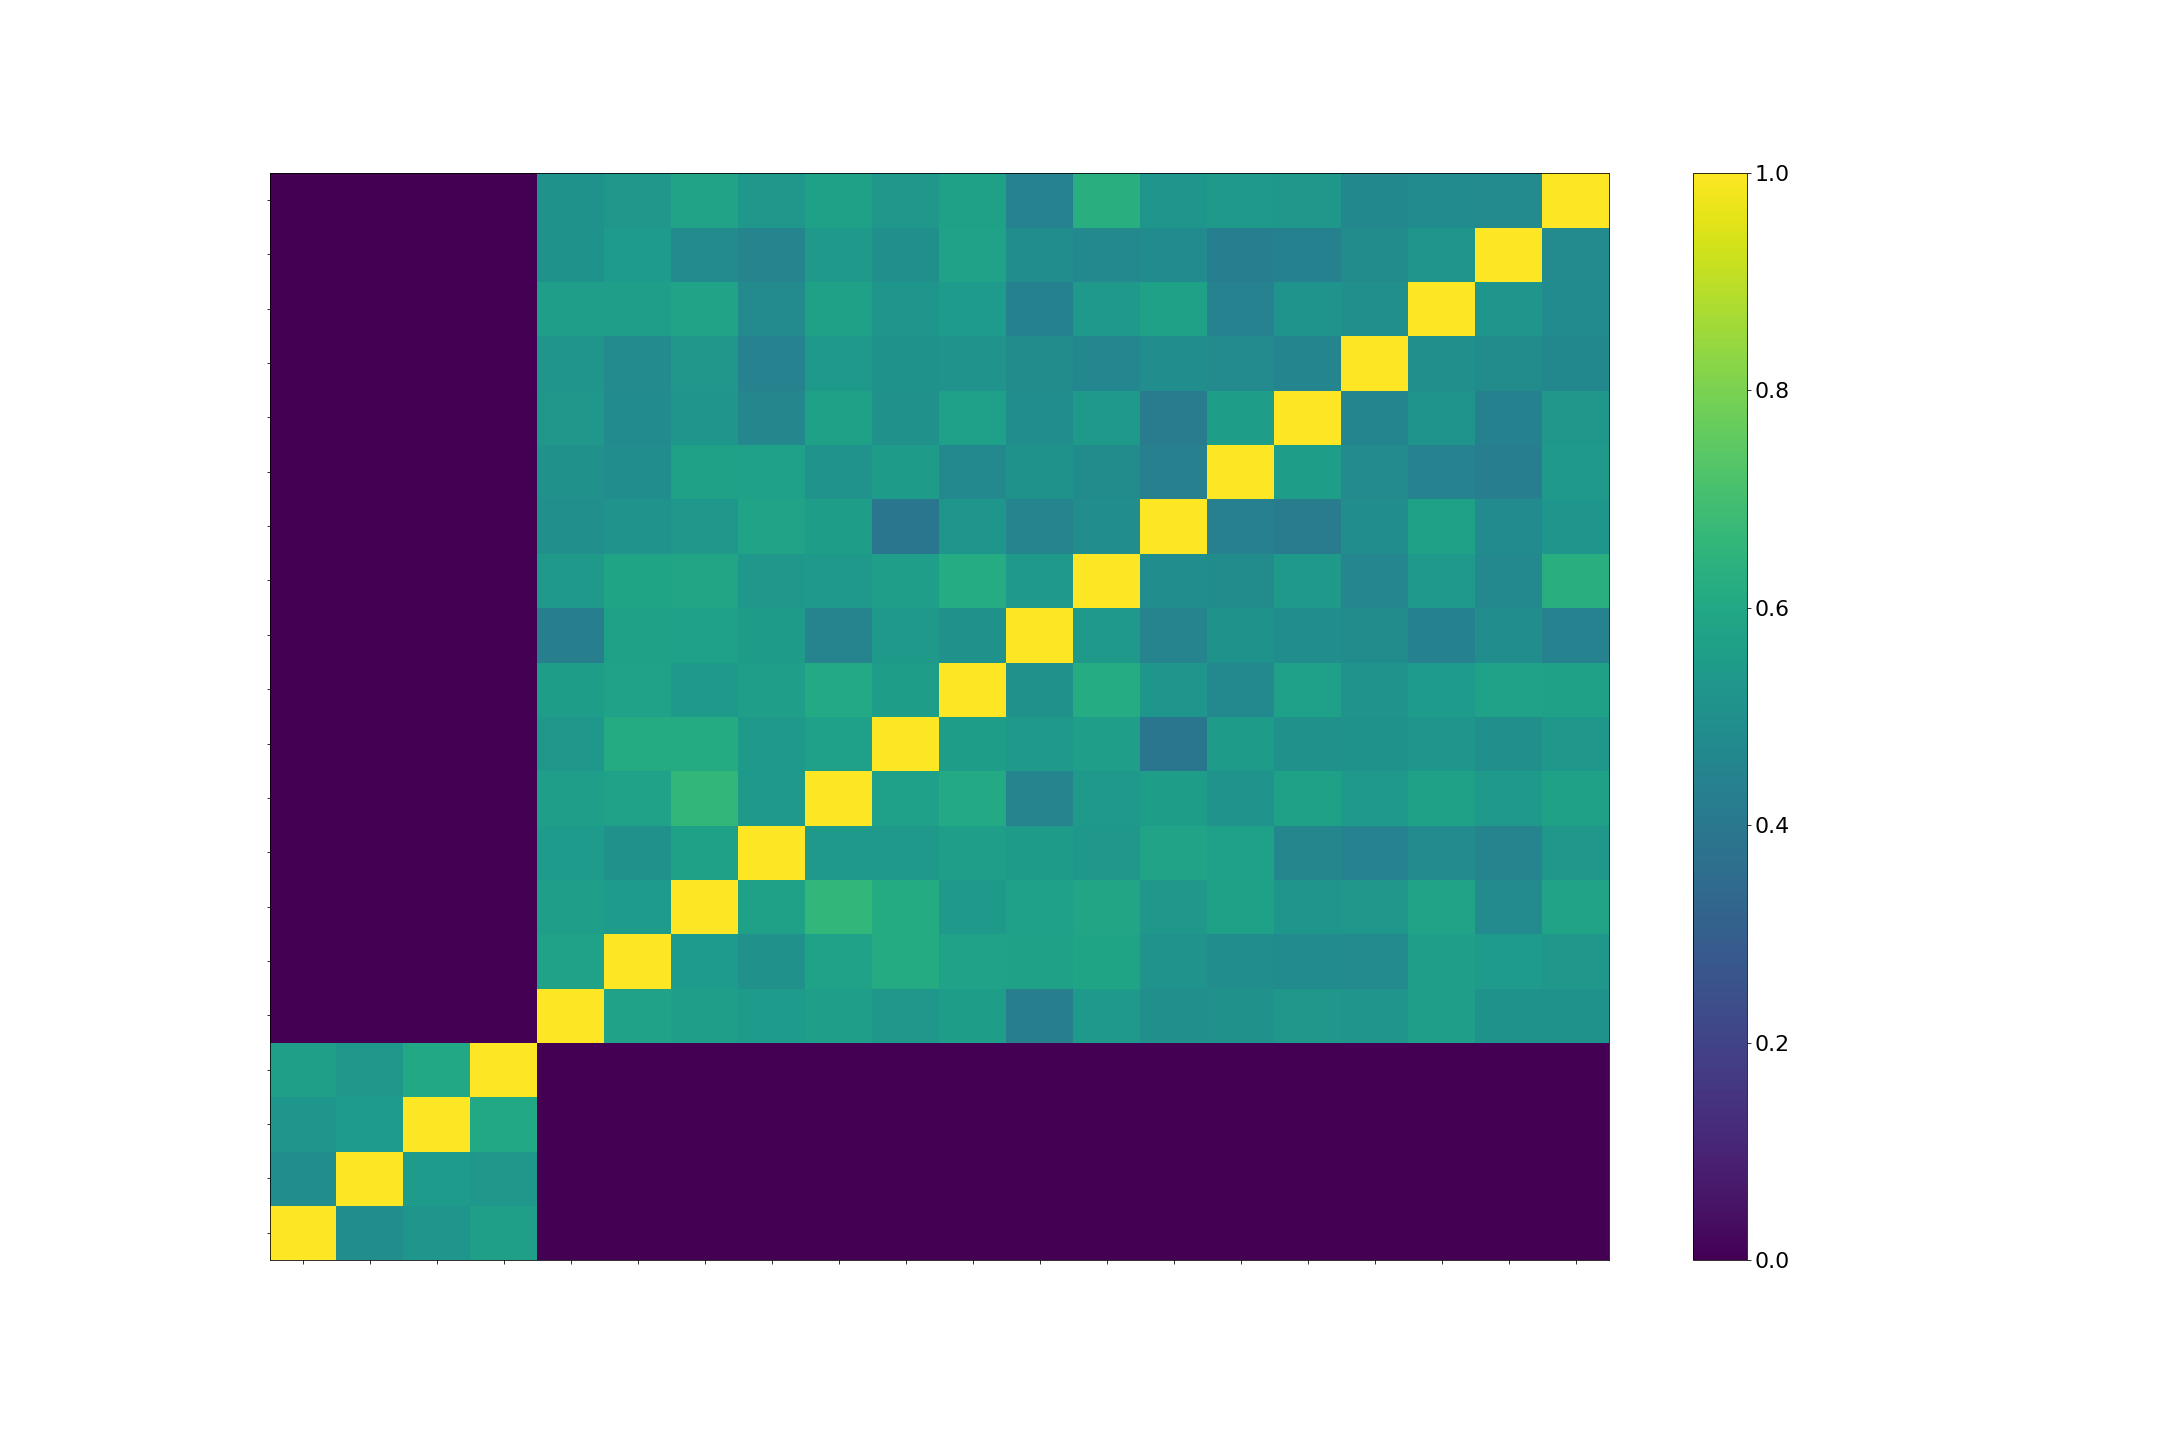
\includegraphics[width = 1.00\textwidth]{BlockCorr.png}
\vspace{-1.75\baselineskip}
\caption{Random Correlation Matrix with 2 blocks}
\label{figRandomCorr}
\end{figure}


This thought experiment brings up a few discussion questions:
\begin{enumerate}
\item Some Industrial stocks perform more similarly to Technology stocks than other Industrials, so why delineate by sector?
\item Within the Technology sector, stocks A and B may perform more similarly to one another and less like stock C, so why not further dissect the stocks within each sector?
\item Why limit the analysis to a portfolio of just Industrials and Technology stocks?
\end{enumerate}
For a more general portfolio, we will generalize this optimization procedure
We refer to this generalized optimal portfolio procedure as Recursive Clustering Risk Parity (RCRP), 
which takes as inputs a covariance matrix $\Sigma$ of returns, and vector $b$. 
In the case of the minimum variance portfolio $b=1$, and $b=\mu$ in the max sharpe ratio portfolio. 
The procedure can be described as follows:
\begin{enumerate}
\item Form the correlation matrix $C$ from the covariance matrix $\Sigma$ for a certain set of instruments $S$.
\item Use advanced unsupervised learning techniques to cluster, and partition $S$ into some optimal $k$ disjoint sets of instruments $S_i$.
\item For each set $S_i$, extract the covariance matrix $\Sigma_i$ and vector $b_i$ associated with those instruments.
\item If $\Sigma_i$ is too small for clustering, find the optimal portfolio vector $w_i$ via the improved approximate inverse portfolio optimization above using $\Sigma_i$ and $b_i$.
Otherwise, recursively set $w_i = RCRP( \Sigma_i, b_i )$. 
Note that $w_i$ has dimension $N_i=|S_i|$ and $1^T w_i = 1$.
\item Using $w_i$ to define the change in basis elements, 
\begin{enumerate}
\item create the compressed covariance matrix $\Sigma^{comp}$ and compressed vector $b^{comp}$ for our portfolio of portfolios. 
This is equivalent to treating the performance of the optimized portfolios as individual instruments. 
Observe that $b_i^{comp}=b_i^T w_i$ and $\Sigma_{ij}^{comp} = w_i^T\Sigma_{ij} w_j$, where $\Sigma_{ij}$ is the submatrix of $\Sigma$ with rows related to instruments in $S_i$ and columns related to instruments in $S_j$.
\item Find the cluster weights vector $v$ via the improved inverse portfolio optimization using $\Sigma^{comp}$ and $b^{comp}$. 
Note that $v$ has dimension $k$, and $1^T v = 1$.
\end{enumerate}
\item For $i = 1, \ldots, k$, set $w_i \to v_i w_i$, then concatenate the weight vectors $w_i$ into a single vector $w$, and return this $w$ as output. Note that $1^Tw=1$ as desired.
\end{enumerate}
For step (2), we consider the ONC algorithm formulated in \cite{LopezAndLewis}, 
though this could be enhanced should improved clustering techniques arise.

This technique reorganizes the index companies as a b-tree of relations, where companies that are highly correlated are “near” one another on the tree, 
while companies that are less correlated are further apart. 
This is consistent with the original premise of HRP, but unlike HRP fully utilizing risk parity at all levels of the tree. 
Furthermore, each non-leaf of the tree does contain 2 or more branches and does not assume equal-sized clusters, thus making it more generalized than the HRP procedure.


\section{Incorporating Limits On Short Positions}\label{sec-LimitShorts}
The above analysis and procedure focused on the scenario where there are no shorting limits. 
In the case of shorting limits, the above process is easily altered to incorporate this modification; we need only modify step (5b).
See Appendix \ref{sec-Appendix2} for proof of the necessary procedure modification.


\section{Notable Alternative Use Cases}\label{sec-AltUseCase}
The previous sections describe how RCRP evaluates $w \propto \Sigma^{-1}\mu$. This is, up to scaling $\lambda$, equivalent to solving $\lambda \Sigma w = \mu$. 
This procedure could be easily modified for use in matrix multiplication by the inverse of the covariance matrix $\Sigma$. 
For example, each column $i$ of $\Sigma^{-1}A$ equals $\Sigma^{-1}A_i$, where $A_i$ is the $i$th column of $A$. 
Similarly, each row $i$ of $B\Sigma^{-1}$ equals $B_i^T\Sigma^{-1}$, where $B_i$ is the $i$th row of $B$.
This is true due to the symmetrical nature of $\Sigma$. 
However, more consideration is necessary for deciding the appropriate $\lambda$ in such scenarios.


\section{Numerical Examples}\label{sec-Simulation}
We now review the financial performance of RCRP. 
For this section, we consider an assortment of industry standard techniques for creating portfolio weights for the minimum variance portfolio, 
and compare the performance of the resulting portfolios from these techniques. 
This analysis focuses on the case with no shorting limits, i.e. where $1^Tw=1$.
The code for this section, written in Python 3, can be found at: \url{https://github.com/mlewis1729}. 
For transparency, there are two modifications made in the code from the source material:
\begin{enumerate}
\item HRP has been ported from Python 2 to Python 3 code using minor syntax modifications
\item The ONC algorithm from \cite{LopezAndLewis} has been
\begin{enumerate}
\item ported from Python 2 to Python 3 code using minor syntax modifications
\item modified in the re-clustering step; where originally the clusters with better than average silhouette t-stats were not re-clustered recursively, 
now only the cluster with the highest silhouette score t-stat is not re-clustered. This slows calculation performance, but ideally improves overall clustering results.
\end{enumerate}
\end{enumerate}
Furthermore, for this section we define the effective number of positions $N_{eff}=\frac{1}{HHI}=\frac{1}{\sum_i w_i^2}$, where HHI is the Herfindahl–Hirschman index\footnote{\HHIURL}.
This metric evaluates how concentrated a portfolio is, as well as the effective number of data points in an exponentially weighted series.
For example, using weights $w_i = (1-\alpha) \alpha^i$ gives us
\[
N_{eff} = \frac{1}{\sum_i w_i^2} = \frac{ 1 - \alpha^2 }{ (1 - \alpha)^2 }.
\]
Given a halflife $H$, we have 
\[
\alpha = \exp(-\epsilon) \Rightarrow \alpha^H = \exp(-H \epsilon ) = \frac{1}{2} = \exp( - \ln 2 ) \Rightarrow \epsilon = \frac{ \ln 2 }{ H }.
\]
This yields $N_{eff} \approx \frac{ 1 - ( 1 - 2 \epsilon ) }{ ( 1 - (1-\epsilon) )^2 } = \frac{ 2 }{ \epsilon } = \frac{ 2 H }{ \ln 2 }$.

The portfolio techniques we consider in this analysis are the following:
\begin{itemize}
\item RCRP, utilizing the extended terms from the inverse variance approximation (where $\rho=\bar{\rho}$) in step 5
\item RCRP, without using the extended terms (equivalent to setting $\bar{\rho}=0$) in step 5
\item HRP
\item the inverse variance portfolio, IVP, 
\item Using Ledoit-Wolf (LW) shrinkage on the empirical covariance matrix
\item Using OAS shrinkage on the empirical covariance matrix
\end{itemize}
The scenario analyzed is as follows: For a given year, e.g. 2020, we fetch the daily returns for a large set of NYSE companies from 3 years back, e.g. 2017, to present. 
On the first day of each month in the chosen year, we use the historical returns up to the end of the previous month to create an empirical covariance matrix. 
In the cases of RCRP, HRP, and IVP we create an exponentially-weighted (EW) covariance matrix with a halflife of 60 days, 
while in the cases of the shrinkage matrices, which aren’t coded to handle EW calculations in the standard libraries in Python, 
we utilize the entire 3+ years of daily returns. 
We then create the optimized portfolio weights using the above techniques, 
and with those portfolios evaluate the realized returns for that given month from the first to the end of that month.
Note that the weights are not allowed to drift, but given these weights are held for a month, the impact from drift should be minimal.
This procedure was run over recent years, specifically 2019-2022.

Figure \ref{fig1} shows the EW moving standard deviation, halflife 20 days, of the realized returns given the above procedures. 
Figure \ref{fig2} shows the same results but normalized by the result for RCRP using the extended terms so as to show relative performance. 
It is readily observable that IVP has the largest volatility, typically performing 2-3x and occasionally 4x worse (average 2.36x) than RCRP. 
HRP performs better than IVP but still typically 1.5x-2.5x worse (average 1.8x) than RCRP. 
The version of RCRP without the extended terms performs slightly worse (1-2x, average 1.35x) than the version with. 
Notably the shrinkage matrix methodologies LW and OAS have more comparable performance (0.5x-1.5x, average 1.2x) to RCRP; 
this may be due to the fact the covariance matrices they use have 3 years (\~750 data points) worth of data, 
while RCRP is effectively using $\frac{2 \cdot 60}{\ln 2} \approx 174$ data points, a byproduct of using exponential weights with halflife 60.
\noindent
\begin{figure}[!h]
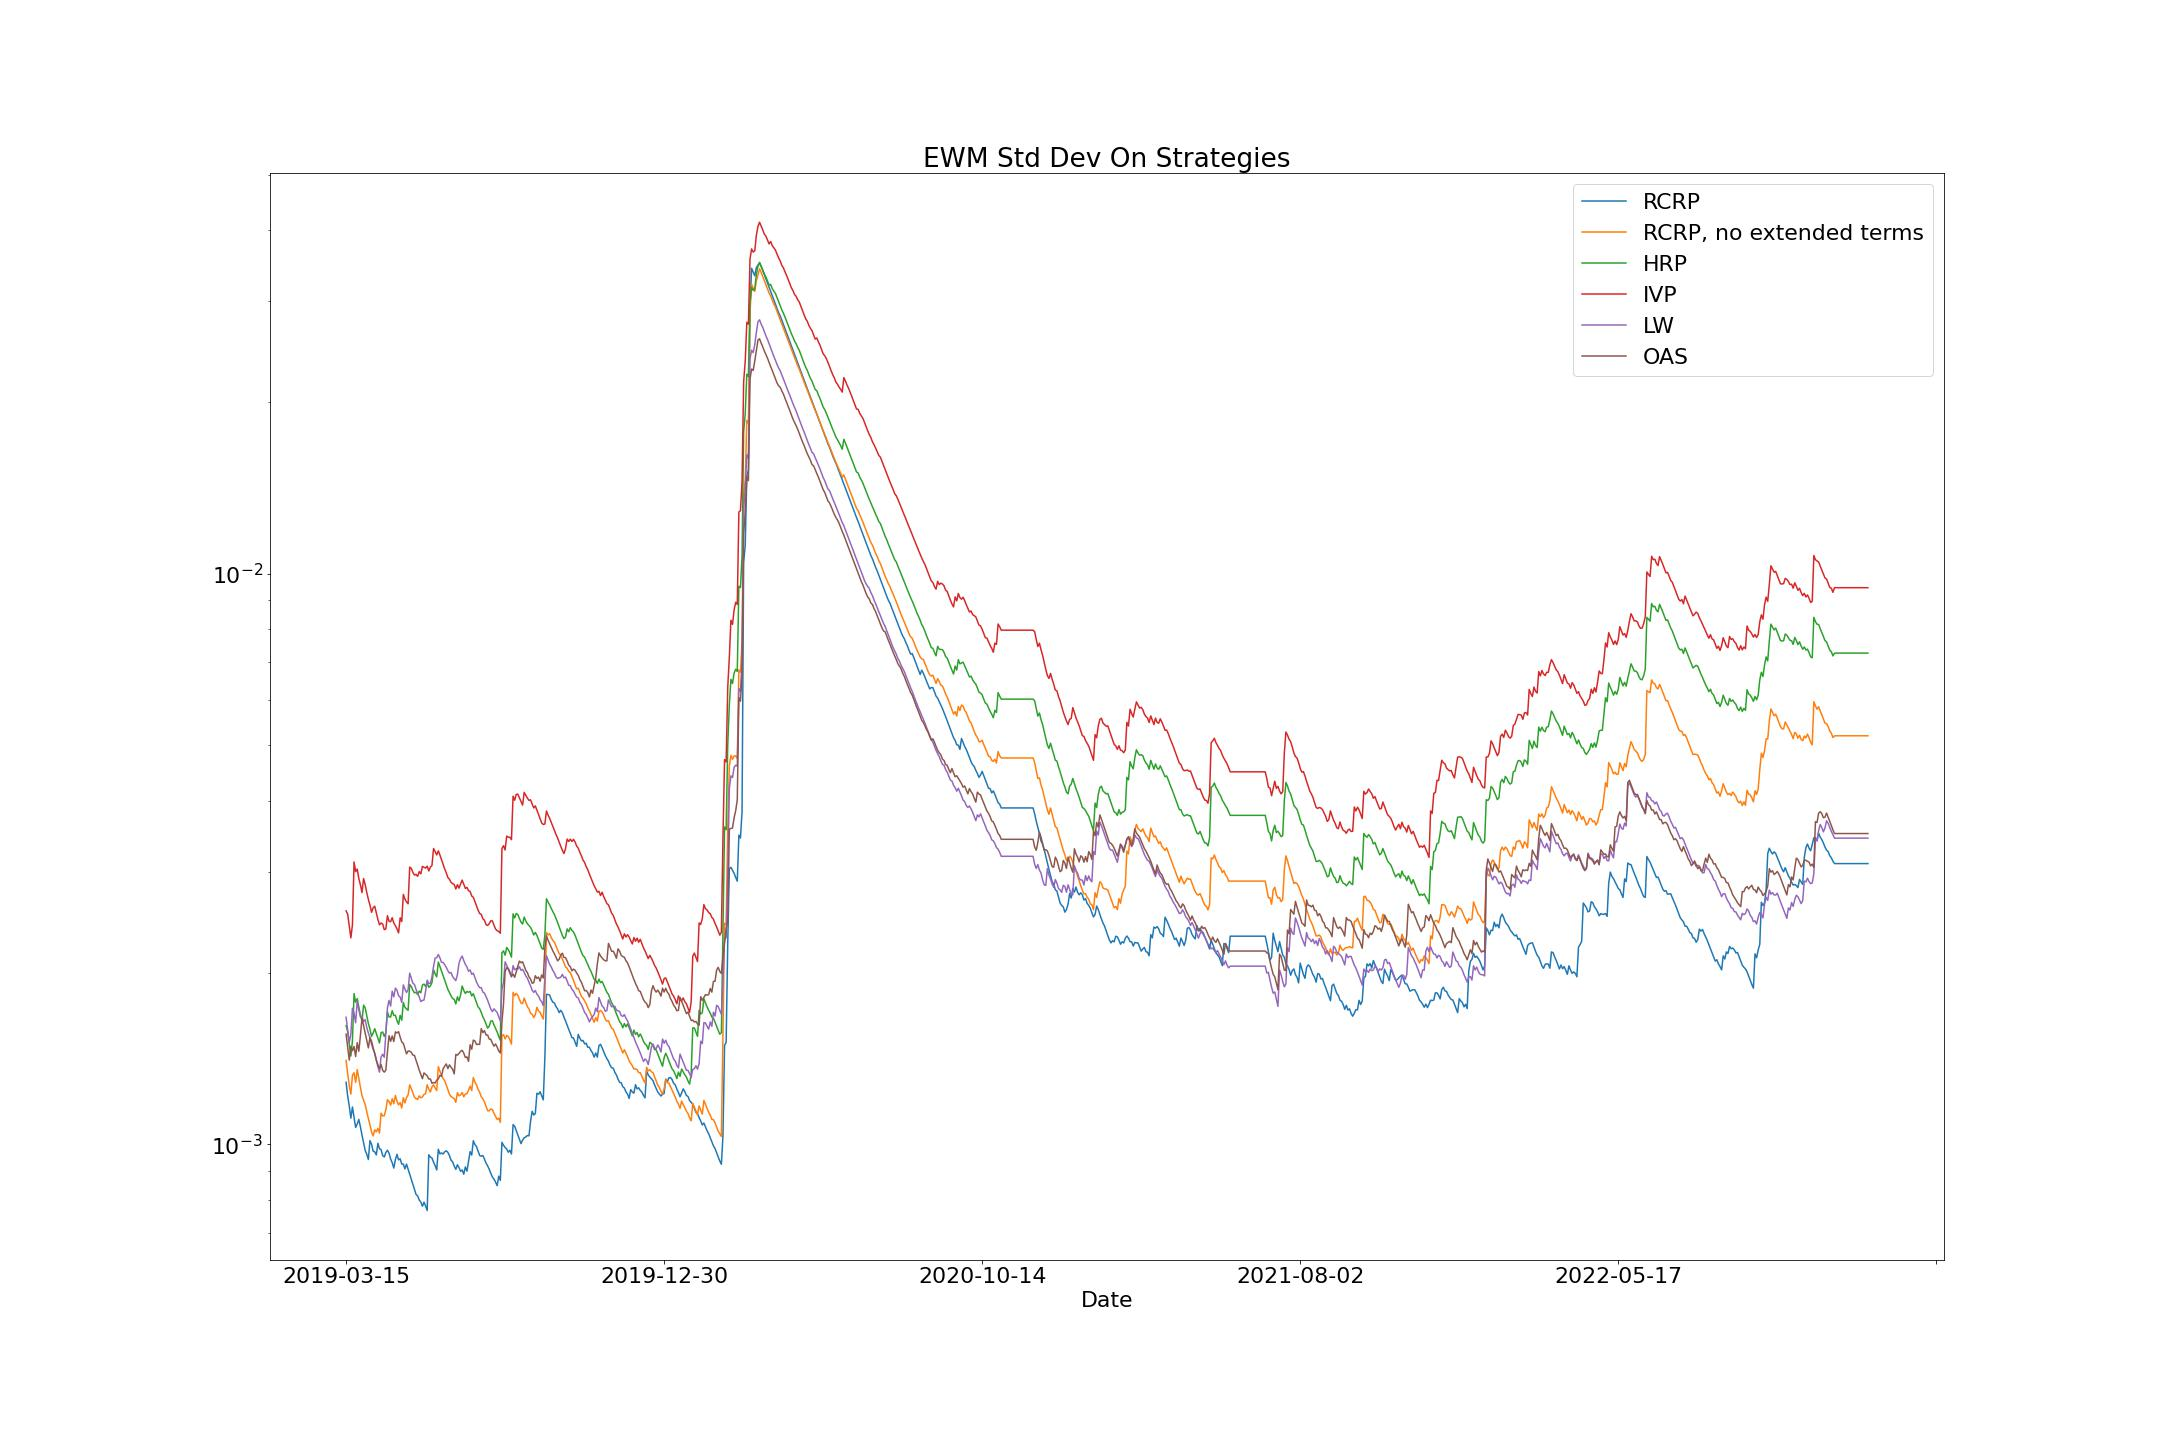
\includegraphics[width = 1.00\textwidth]{image1.jpg}
\vspace{-1.75\baselineskip}
\caption{EW moving standard deviation of daily returns of strategies, HL=20}
\label{fig1}
\end{figure}

\noindent
\begin{figure}[!h]
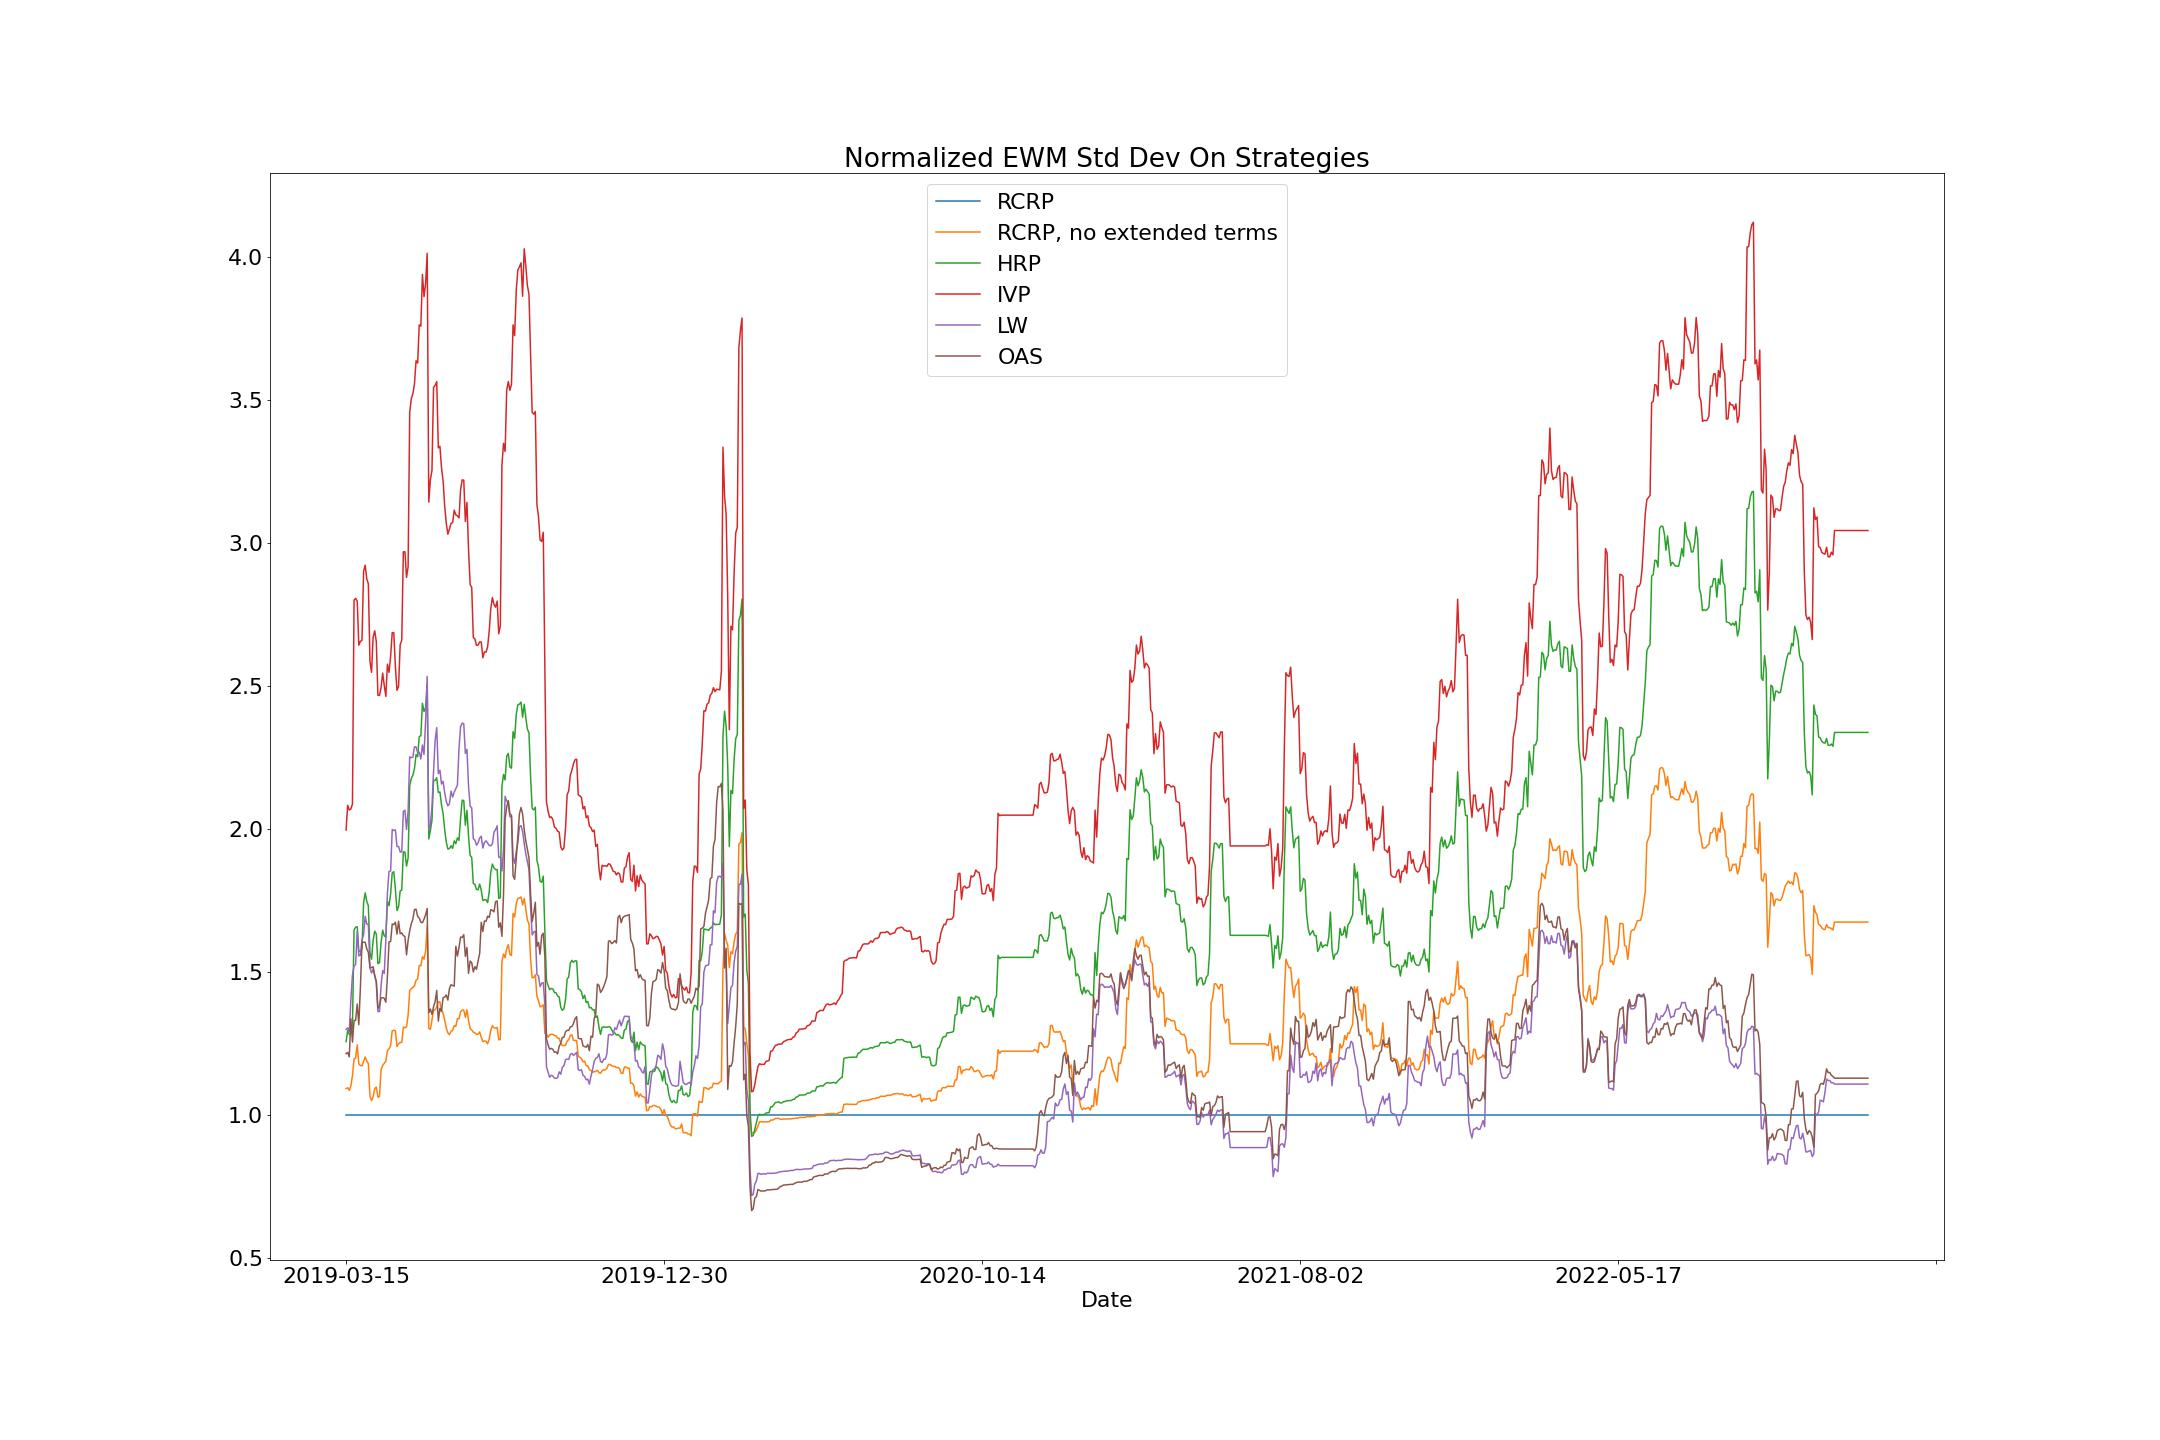
\includegraphics[width = 1.00\textwidth]{image2.jpg}
\vspace{-1.75\baselineskip}
\caption{Normalized EW moving standard deviation of daily returns of strategies, HL=20}
\label{fig2}
\end{figure}

Given the portfolio weights, Figure \ref{fig3} shows the effective number of positions in each portfolio over time. 
From this we see that IVP has the largest effective number of positions ($\sim 480$), and thus lowest concentration in the portfolio, 
while HRP comes in second with a slightly lower effective position size ($\sim 200$). 
The shrinkage matrix techniques come in the middle of the pack (LW $\sim 130$, OAS $\sim 60$) 
while RCRP with extended terms comes in the most concentrated at $\sim 20$ positions. 
RCRP without the extended terms shows up in between the shrinkage matrix techniques with roughly 75 positions on average.
%Chart 3: Effective Number of Positions
\noindent
\begin{figure}[!h]
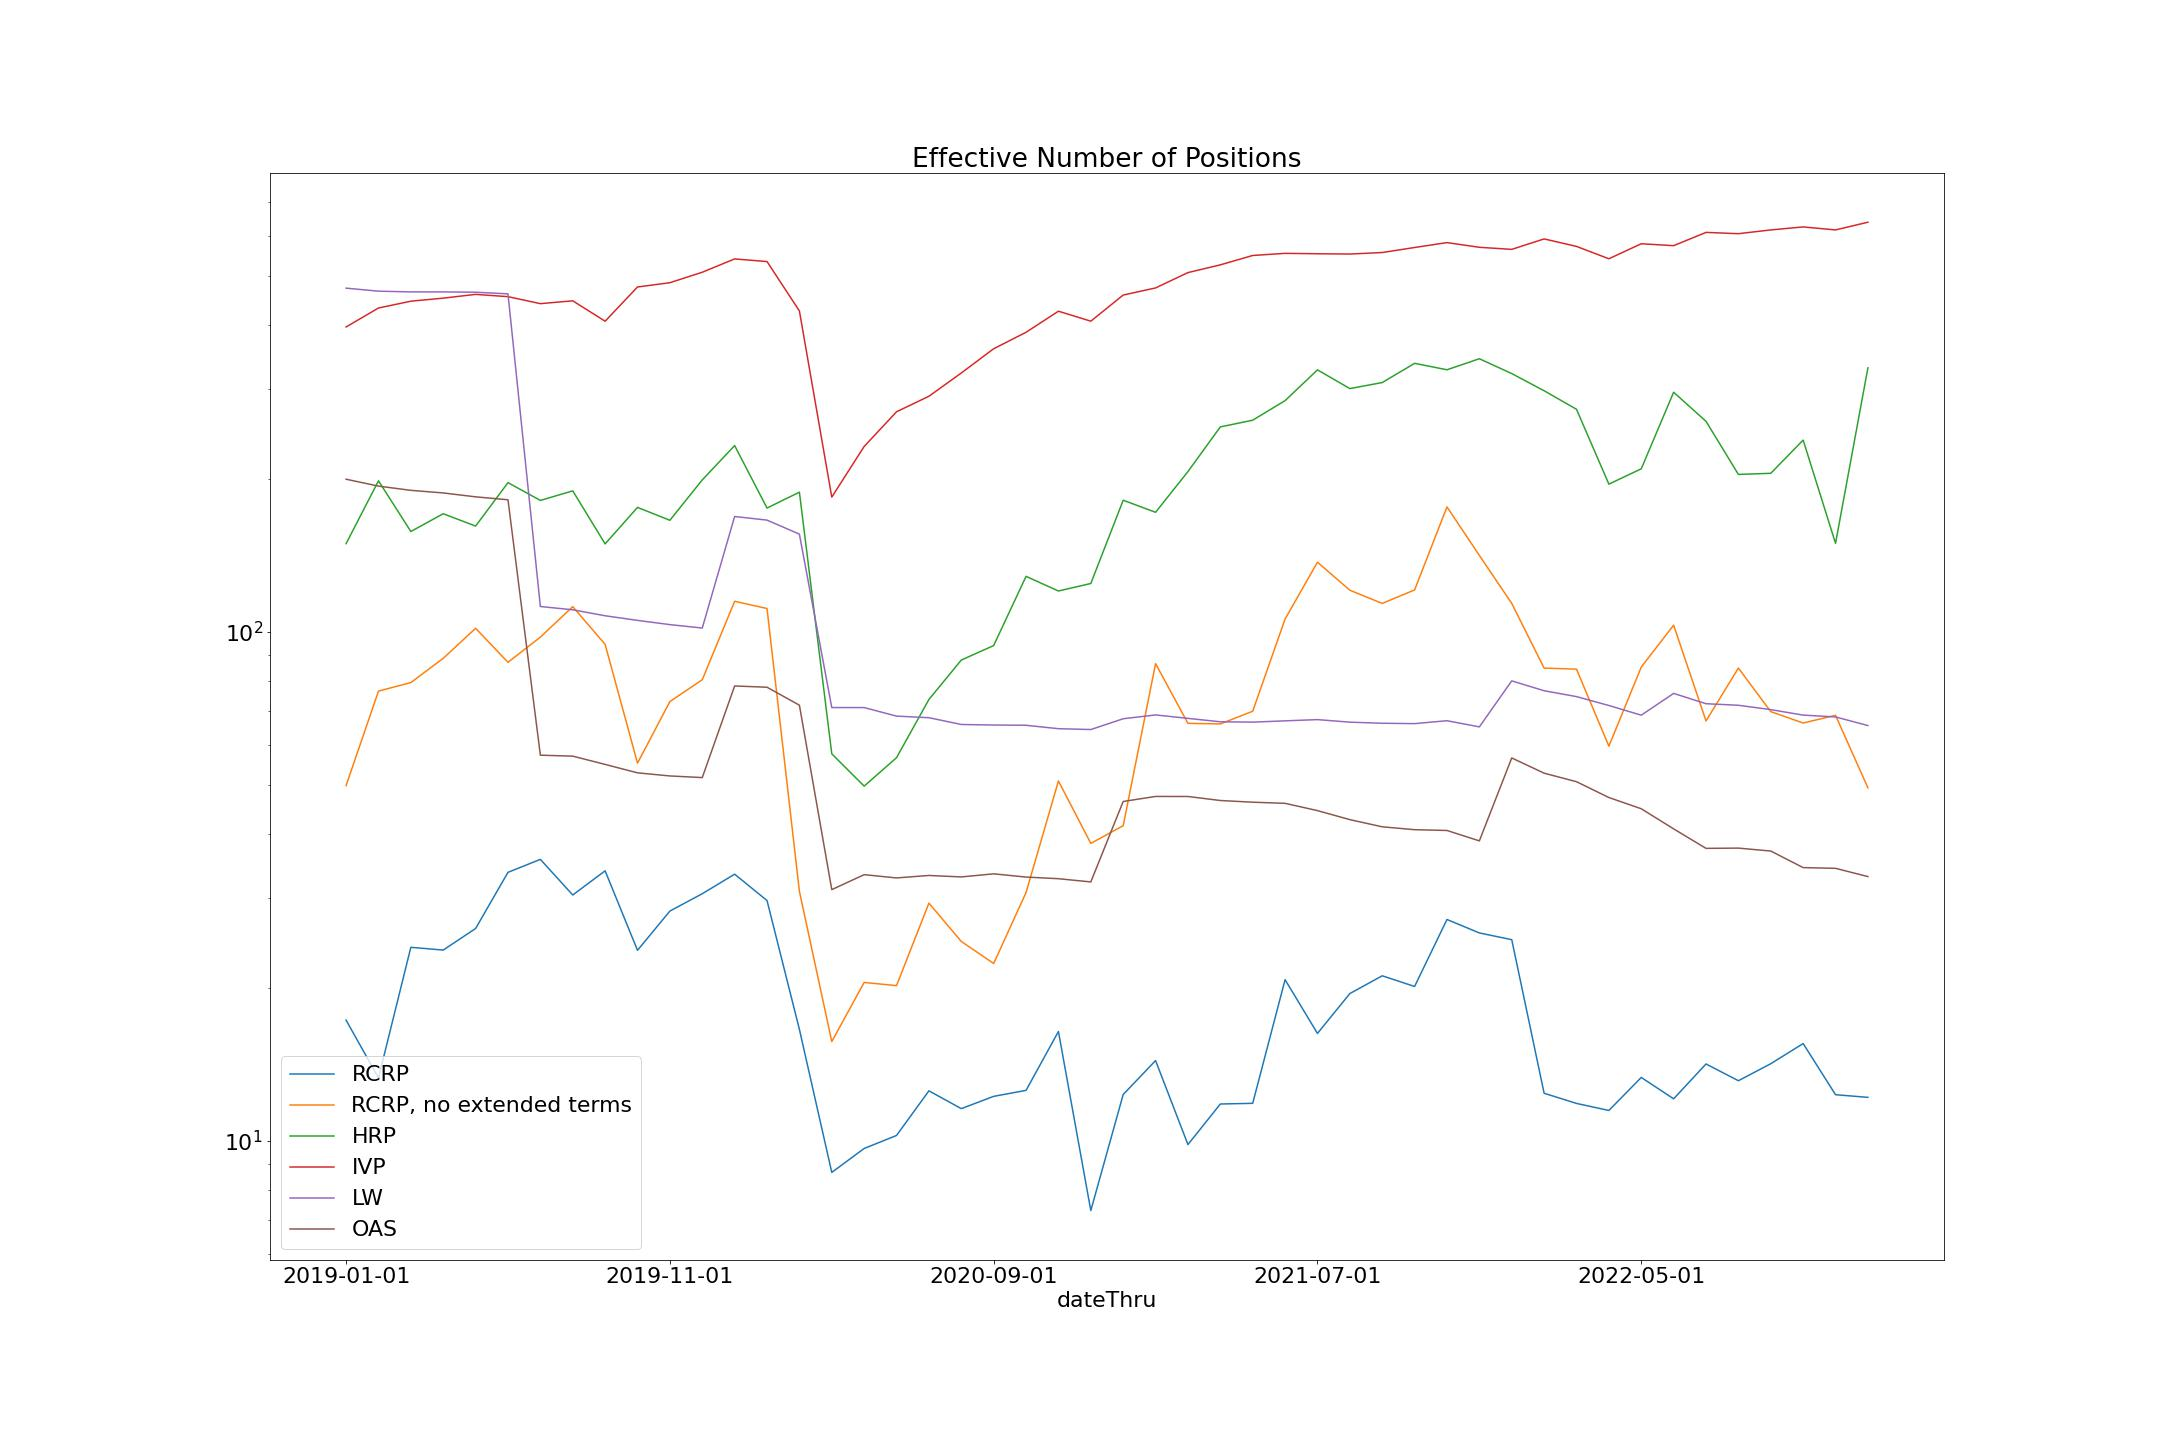
\includegraphics[width = 1.00\textwidth]{image3.jpg}
\vspace{-1.75\baselineskip}
\caption{Effective Number of Positions}
\label{fig3}
\end{figure}
An alternative metric for analyzing portfolio concentration is the maximum absolute weight at any given time. 
This is shown in Figure \ref{fig4}. 
As with Figure \ref{fig3}, we observe RCRP with extended terms is the most concentrated, 
with the largest position typically around 14\%, while RCRP without the extended terms is typically half that ($\sim7$\%). 
HRP comes in third at roughly 3.2\%, while LW, OAS, and IVP hold positions no larger than 1-2\% on average.
%Chart 4: Max Absolute Weight
\noindent
\begin{figure}[!h]
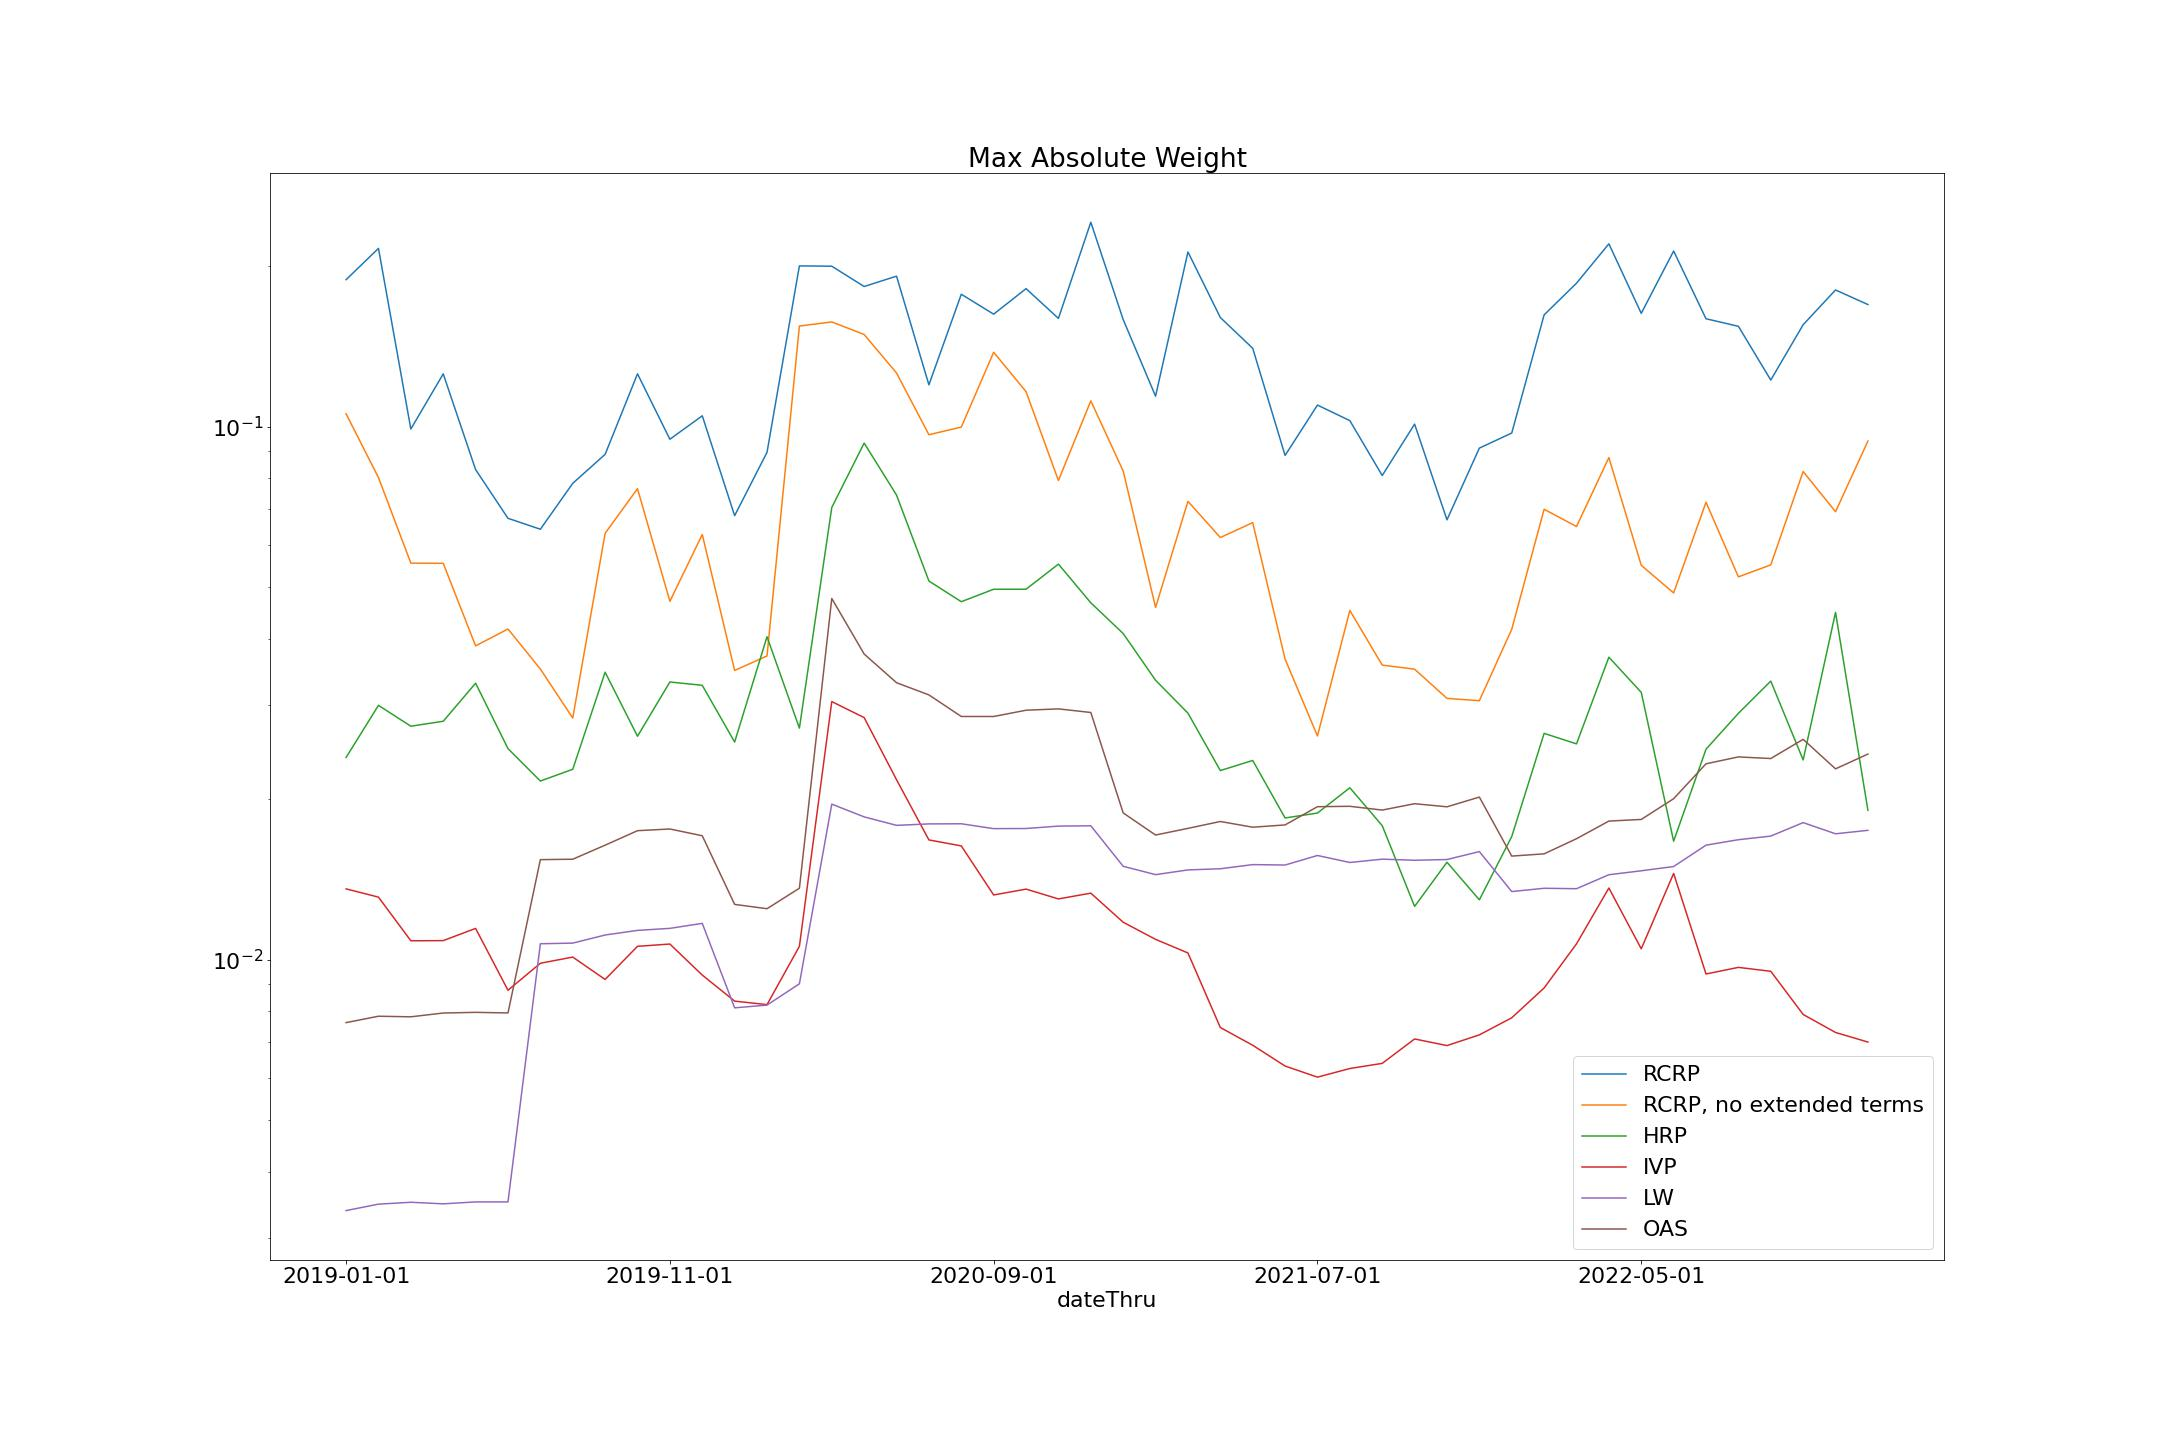
\includegraphics[width = 1.00\textwidth]{image4.jpg}
\vspace{-1.75\baselineskip}
\caption{Max Absolute Weight}
\label{fig4}
\end{figure}
For completeness, we also include a chart with total number of positions, 
which is to say number of positions where weights are non-zero. 
This is shown in Figure \ref{fig5}. 
For this analysis, we are typically considering 1000-1600 companies.
%Chart 5: Total Number of Positions
\noindent
\begin{figure}[!h]
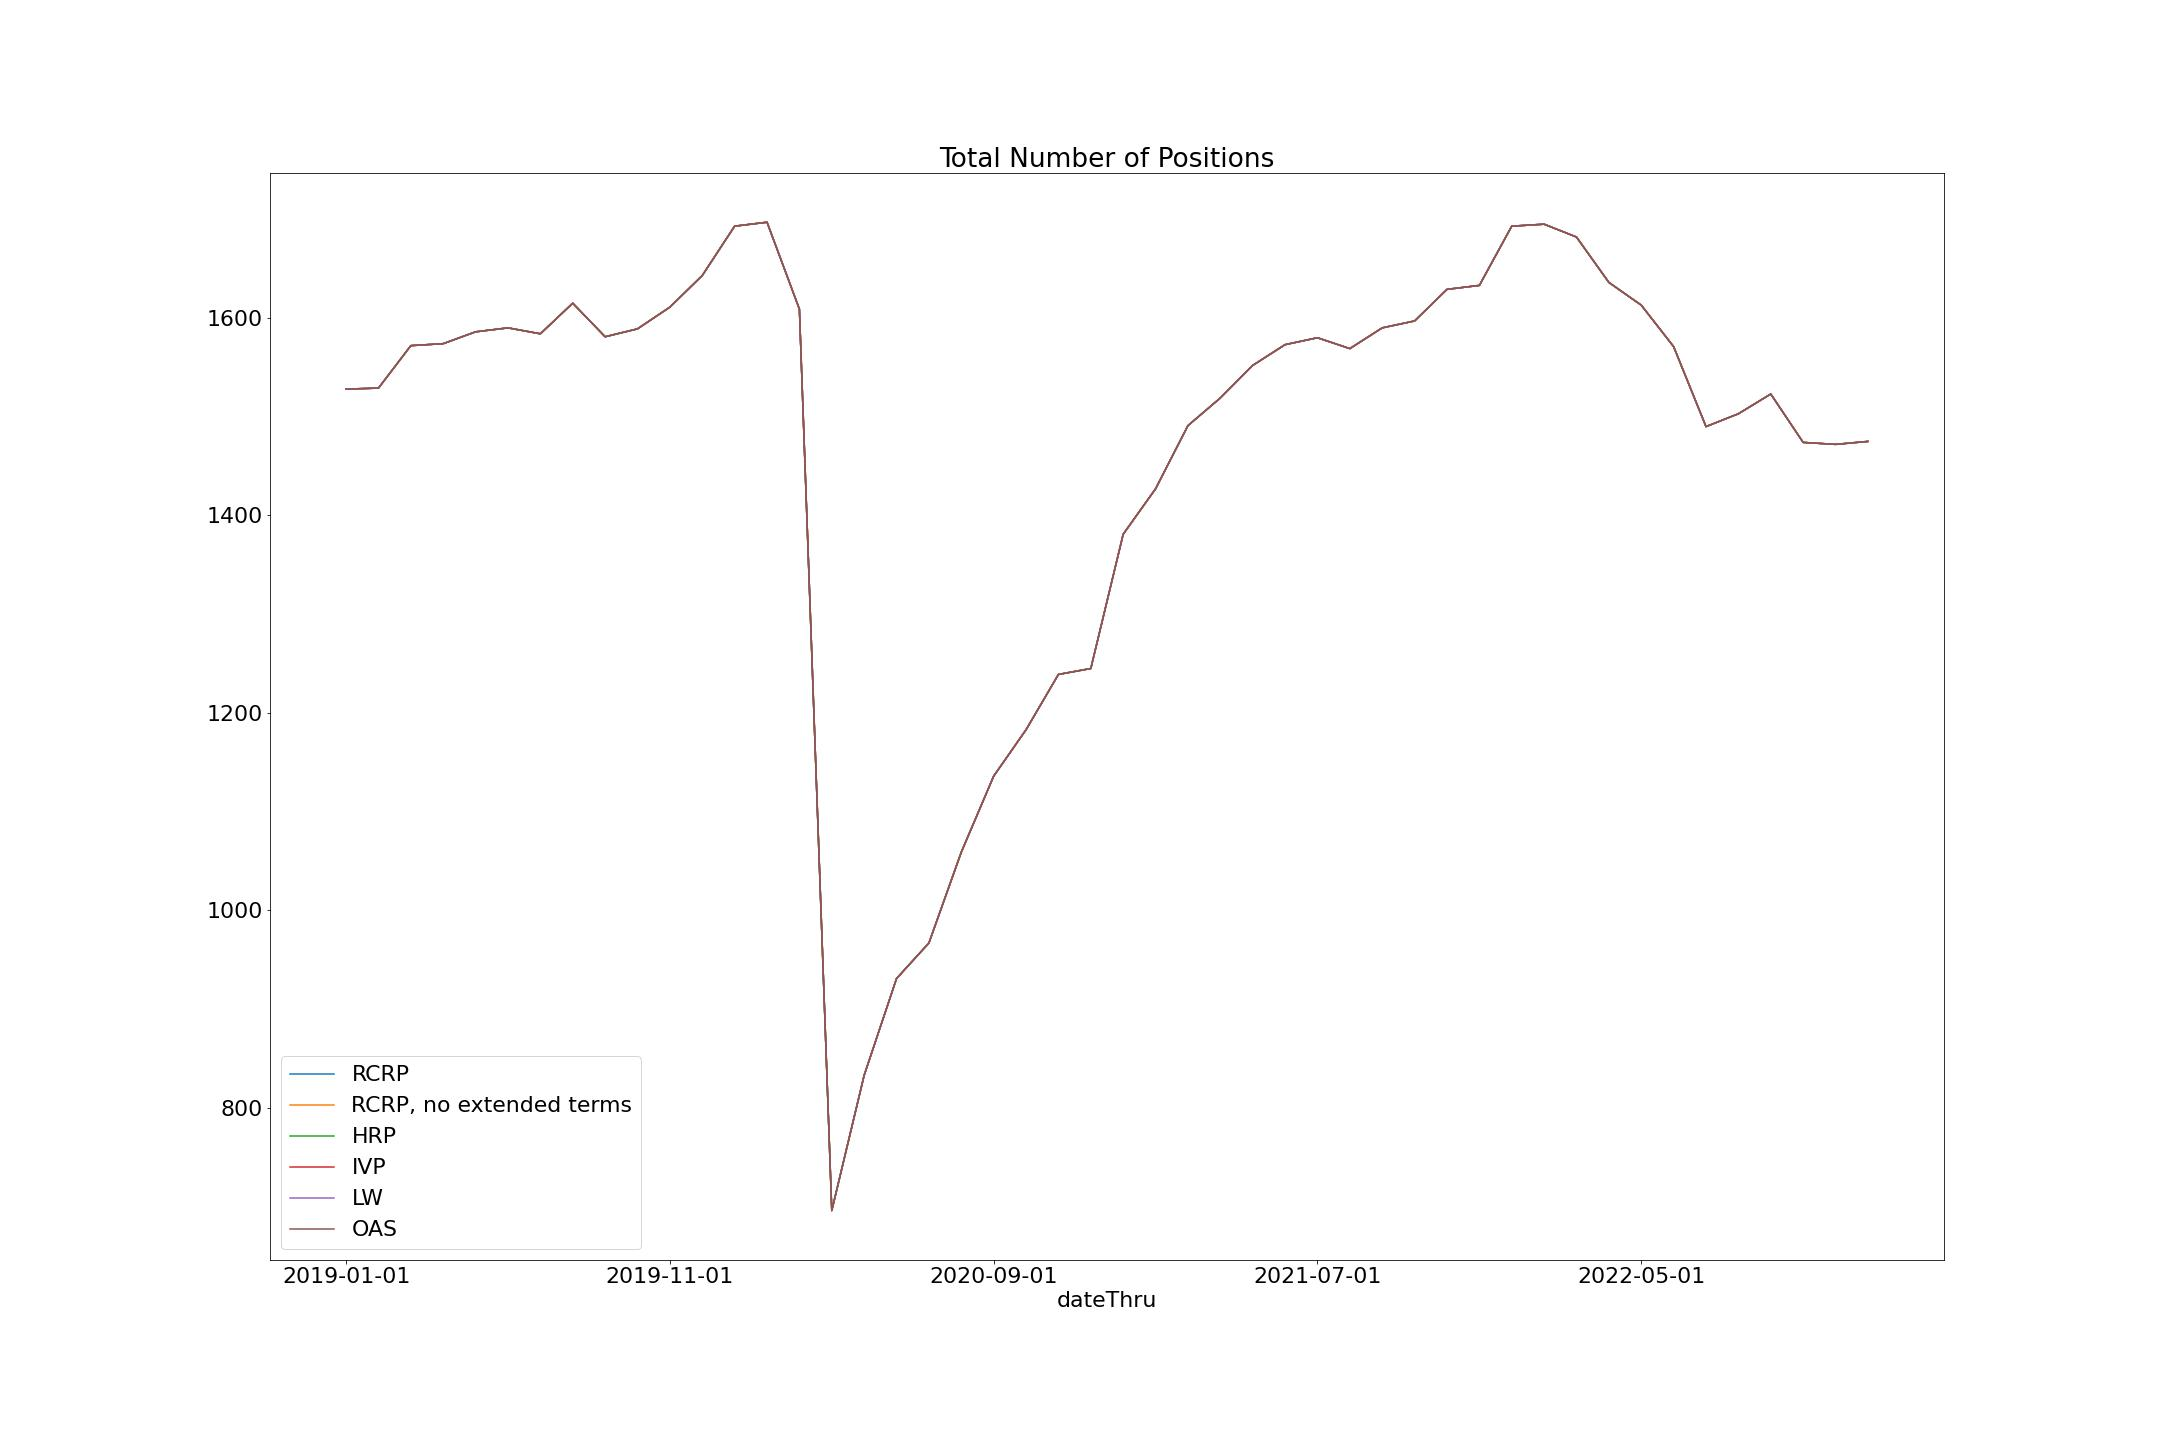
\includegraphics[width = 1.00\textwidth]{image5.jpg}
\vspace{-1.75\baselineskip}
\caption{Total Number of Positions}
\label{fig5}
\end{figure}

\section{Conclusions}\label{sec-Conclusions}
This new procedure RCRP is designed to perform optimal portfolio calculations without the need for the often numerically unstable procedure of inverting the covariance matrix. 
RCRP builds on the original principles of HRP, while ensuring the original correlations of the companies are adhered to more thoroughly by designing a b-tree of relationships between the companies. 

We observe that RCRP more effectively lowers the volatility of a portfolio than HRP or IVP, 
and even on average performs better than standard shrinkage matrix methodologies despite having significantly fewer data points. 
One notable concern is an increased concentration in the portfolio, 
a concern that is somewhat mitigated by not using the extended terms in the inverse approximating step, 
but which comes at the cost of reduced performance. 
Further testing would be necessary to better delineate this tradeoff.

\appendix
\section{Optimal Max Sharpe Portfolios}\label{sec-Appendix1}
In \cite{HRP}, a proof is given for the optimal minimum variance portfolio construction. 
The following proof for the optimal max sharpe portfolio construction is given for completeness. 
A similar proof is given in \cite{StackExchange}.

Our goal is to solve
\begin{equation*}
\begin{aligned}
\argmax_{w} \quad & \frac{w^T \mu}{ \sqrt{ w^T \Sigma w } } \\
\textrm{s.t.} \quad & 1^T w = 1\\
\end{aligned}
\end{equation*}
Let
\begin{equation*}
\begin{aligned}
g_1( w ) \quad & = w^T \mu \\
g_2( w ) \quad & = w^T \Sigma w \\
h( x_1 , x_2 ) \quad & = \frac{x_1}{ \sqrt{ x_2 } } \\
f( w ) \quad & = \frac{ w^T\mu}{ \sqrt{ w^T \Sigma w } } = h( g_1(w),g_2(w)) \\
\end{aligned}
\end{equation*}
We set the derivative of $f(w)$ to $0$, and find
\begin{equation*}
\frac{1}{\sqrt{w^T \Sigma w}} \mu_i - \frac{ w^T \mu }{ 2(w^T \Sigma w)^{3/2} } ( 2\Sigma w)_i = 0 \textrm{ } \forall i \Rightarrow \Sigma w = \frac{ w^T \Sigma w }{ w^T \mu } \mu = C \mu \\
\end{equation*}
implying the optimal portfolio $w = C\Sigma^{-1}\mu$. 
Observe that $f(w)=f(Cw)$ for $C>0$; thus, the optimal max sharpe portfolio has $w \propto \Sigma^{-1}\mu$. 
Note that this same argument extends to the case where short positions are limited, 
in which case the condition $\sum_i |w_i| = 1$ holds. 
Thus, the max sharpe portfolio with no shorting limits differs from the case with limits only by the normalization.

\section{Optimal Min Variance Portfolios With Shorting Limits}\label{sec-Appendix2}
We now discuss the scenario where short positions on the portfolio are limited. 
To do so, we exchange the condition $\sum_i w_i = 1$ with $\sum_i |w_i| = 1$.
Section \ref{sec-Appendix1} makes clear the max sharpe ratio portfolio with shorting limits differs only in normalization from the case without limits. 
In this section, we focus our attention on the minimum variance portfolio.

We consider the problem
\begin{equation}
\begin{aligned}
\argmin_{w} \quad & w^T \Sigma w \\
\textrm{s.t.} \quad & \sum_i |w_i| = 1\\
\end{aligned}
\end{equation}
Using Lagrange multipliers, we set the derivative of $w^T \Sigma w + \lambda ( \sum_i |w_i| - 1 )$ to $0$, and find
\[
\Sigma w = Cs \Rightarrow w = C\Sigma^{-1}s,
\]
where $s_i = \sigma(w_i)$, the sign of $w_i$, 
and $C$ is a normalizing constant. 
Observe that $s^T w = \sum_i |wi| = 1 = Cs^T\sigma^{-1}s$, 
and thus $C = \frac{1}{s^T\Sigma^{-1}s}$. 
Therefore, our optimal minimum variance portfolio is $w = \frac{\Sigma^{-1}s}{s^T\Sigma^{-1}s}$, 
and the minimum variance is $w^T \Sigma w = C^2 s^T \Sigma^{-1}\Sigma \Sigma^{-1}s = C$.

The difficulty of this problem depends on discovering the appropriate $s$. 
However, interpreting $C$ is far simpler, as it is the smallest variance it can be, so we focus our attention on that. 
Let $S = \{s | s_i \in \{-1,1\} \textrm{ } \forall i \}$ be the set of all possible sign vectors, 
and thus $s \in S$. 
Thus, our problem reduces to finding
\[
\argmax_{s\in S} s^T \Sigma^{-1} s.
\]
This is challenging to analyze for general covariance matrix $\Sigma$, 
so we reduce our consideration to the approximate matrix listed earlier, 
namely
\[
\Sigma = (1-\rho) \Sigma_{diag} + \rho \sigma \sigma^T.
\]
Note that $\Sigma$ is positive semi-definite. 
By the Matrix determinant lemma,
\[
\operatorname{det}(\Sigma) = \operatorname{det}( (1-\rho)\Sigma_{diag}) \left( 1 + \frac{\rho \sigma^T \Sigma_{diag}^{-1} \sigma}{1-\rho} \right) \geq 0 \Rightarrow \frac{\rho \sigma^T \Sigma_{diag}^{-1} \sigma}{1-\rho} = \frac{ N\rho}{1-\rho} \geq -1 ,
\]
implying that $\rho \geq \frac{-1}{N-1}$ is a necessary condition. 
Next, observe that $s^T \Sigma_{diag}^{-1} s = \sum_i \frac{1}{ \sigma_i^2 } \forall s \in S$. 
Third, let $K = \frac{\rho}{ 1+ \rho (N-1) }$, and thus $\sigma(K)= \sigma(\rho)$. 
Given that
\[
\Sigma^{-1} = \frac{1}{1 - \rho} \Sigma_{diag}^{-1} - \frac{ \rho }{ (1-\rho) (1 + \rho (N-1) ) } \left( \frac{1}{\sigma} \right) \left( \frac{1}{\sigma} \right)^T
\]
we find
\[
s^T \Sigma^{-1} s = \frac{1}{1-\rho} \left( \sum_i \frac{1}{\sigma_i^2} \right) - \frac{K}{1-\rho} \left( \left( \frac{1}{\sigma} \right)^T s \right)^2
\]
If $\rho < 0$, then $K<0$, and thus maximizing $s^T \Sigma^{-1} s$ 
requires maximizing $| \left( \frac{1}{\sigma} \right)^T s |$. 
Given that $\sigma_i>0 \textrm{ } \forall i$, the optimal $s = \pm 1$. 
If $\rho > 0$, then $K > 0$, 
and thus maximizing $s^T \Sigma^{-1} s$ requires minimizing $| \left( \frac{1}{\sigma} \right)^T s |$.

Since $s$ is a vector of $\pm$1s, we see that minimizing $| \left( \frac{1}{\sigma} \right)^T s |$ 
can be observed as the optimization version of the partition problem, though with real numbers rather than integers, 
which is known to be NP-hard \cite{NPComplete}. 
For small $N$, we can check all $s \in S$, noting that $|S|=2^N$. 
For improved computation, note that the variance is the same for $\pm s$; 
therefore, consider only $s$ such that $s_1=1$, 
thereby reducing computation by a factor of 2. 
For larger $N$, an approximate solution must be found.

Consider the following greedy algorithm: let $s_1=1$, 
and let $y= \frac{1}{\sigma_i}$ hold the running sum. 
For $n > 1$, if $y>0$, then set $s_n = -1$, 
and $ y \leftarrow y - \frac{1}{\sigma_n}$; 
otherwise, set $s_n=1$, and $y \leftarrow y + \frac{1}{\sigma_n}$. 
When $n=N$, observe that $y=\sum_j \frac{ s_j }{ \sigma_j }$. 
We can then repeat this greedy procedure multiple times by permuting 
the $\sigma_i$, running this procedure, performing the inverse permutation 
on the resulting $s$, and ultimately choose the $s$ that obtains 
the smallest $|y|$.

Finally, there is the matter of confirming that, given the optimal $s$, 
the condition $s_i =  \sigma(w_i)$ is satisfied. 
Given that $w = C\Sigma^{-1}s$, and $C>0$, we observe
\begin{equation*}
\begin{aligned}
w_i &\propto \frac{ s_i }{ \sigma_i^2 } - \frac{ K }{ \sigma_i } \sum_j \frac{ s_j }{ \sigma_j } \\
\Rightarrow & | w_i | = s_i w_i \propto \frac{ 1 }{ \sigma_i^2 } - \frac{ K s_i }{ \sigma_i } \sum_j \frac{ s_j }{ \sigma_j } \geq 0 \\
\Rightarrow & \frac{ 1 }{ \sigma_i } - K s_i \sum_j \frac{ s_j }{ \sigma_j } \geq 0 \\
\end{aligned}
\end{equation*}
is a necessary and sufficient condition. We see this condition is 
trivially satisfied when $\rho < 0 \Rightarrow K<0$, 
with optimal $s=\pm 1$. 
Observe that $\rho \in [0,1] \Rightarrow K \in \left[ 0,\frac{1}{N} \right]$. 
If $s_i \sum_j \frac{s_j}{ \sigma_j} \leq 0$, 
then this condition is satisfied trivially; 
therefore, consider the case $s_i \sum_j \frac{ s_j }{ \sigma_j} \geq 0$.
Observe that, if $s_i \geq 0$, then $\sum_j \frac{s_j}{ \sigma_j} \geq 0$.
In this scenario, if $\sum_j \frac{s_j}{ \sigma_j} \geq \frac{1}{\sigma_i}$,
the sum could be decreased by setting $s_i=-1$, 
and thus is not the optimal $s$. 
Consequently, in this scenario, $\sum_j \frac{s_j}{ \sigma_j} < \frac{1}{\sigma_i}$, 
and thus the condition $K s_i \sum_j \frac{s_j}{\sigma_j} \leq \frac{1}{\sigma_i}$ is satisfied. 
A similarly argument confirms the case for $s_i<0$, and thus we confirm the condition 
$s_i=\sigma(w_i)$ is satisfied for optimal s.


\begin{thebibliography}{9}
\bibitem{HRP}
L\'opez de Prado, Marcos, Building Diversified Portfolios that Outperform Out-of-Sample (May 23, 2016). Journal of Portfolio Management, 2016; \url{https://doi.org/10.3905/jpm.2016.42.4.059}. 
Available at SSRN: \url{https://ssrn.com/abstract=2708678} or \url{http://dx.doi.org/10.2139/ssrn.2708678}
%%
\bibitem{LopezAndLewis}
L\'opez de Prado, Marcos and Lewis, Michael J., Detection of False Investment Strategies Using Unsupervised Learning Methods (August 18, 2018). 
Available at SSRN: \url{https://ssrn.com/abstract=3167017} or \url{http://dx.doi.org/10.2139/ssrn.3167017}
%%
\bibitem{StackExchange}
Vim (\url{https://quant.stackexchange.com/users/19004/vim}), Maximum Sharpe portfolio (no short selling restrictions) 
Quantitative Finance Stack Exchange, URL: \url{https://quant.stackexchange.com/questions/43999/maximum-sharpe-portfolio-no-short-selling-restrictions} (version: 8/26/2019)
%%
\bibitem{NPComplete}
Garey, M. R. and Johnson, D. S., Computers and Intractability. A Guide to the Theory of NP-Completeness (1979).
%%
%\bibitem{HHI}
%Herfindahl–Hirschman index, Wikipedia (September 20, 2023), URL: \url{https://en.wikipedia.org/wiki/Herfindahl%E2%80%93Hirschman_index#Effective_assets_in_a_portfolio}
\end{thebibliography}

\end{document}

